\chapter{Introduction}
For millennia, Man has turned his gaze skyward in awe and wonder at the heavens and wondered at the processes that processes that drive structure on the colossal scale of galaxies and galaxy clusters. As physicists we conduct experiments to better out understanding of the processes and laws that control the universe; an old joke goes that as astronomers, our experiment has already been conducted for us, it's called The Big Bang: our job is to use it to test the theories and laws of physics. Indeed, astronomy is a unique opportunity to test our knowledge as scales and limits that are not attainable here on Earth.

% Need to update textgreek package once version 20170724-1 is marked as stable.
The most successful cosmological description of the universe is the dark energy (famously introduced by Einstein to maintain a steady-state universe and represented by \textLambda), cold dark matter ({\textLambda}CDM) \citep{Peebles1982, Bond1982, Blumenthal1982, Blumenthal1984} coupled with inflation \citep{Guth1981}. This describes how the current state of the universe (68.3\% Dark Energy (currently best described with a scalar field), 26.4\% cold dark matter (a matter-like species which only interacts gravitationally), $\sim$4.9\% ordinary baryonic matter and $<$0.003\% radiation \citep{PlanckCollaboration2016}, complete with deep gravitational potential wells in which galaxies and galaxy clusters have formed) has evolved from an infinite and random spacetime 'foam'. Quantum fluctuation within this 'foam' cause region to form which has the corrected conditions for inflation to occur: this includes a quantum scalar field with a sufficient energy density to dominate the region \citep{Linde1982, Albrecht1982}. This field cause the exponential expansion of space at superluminal speeds. Quantum fluctuations are rapidly expanded to beyond the scale of the horizon (distance that a massless particle can travel within the age of the universe). At this point they become frozen in as perturbation to the density profile of the universe (any perturbations prior to the start of inflation are stretched so thin that they can be considered completely negligible). Once the energy density of the inflationary field becomes too low, inflation ends, radiation dominates and the expansion slows to subluminal speeds. As the horizon expands at the speed of light, the density perturbations re-enter the horizon (smallest first), providing seed for the gravitational collapse of dark matter. This process has hardwired hierarchical growth of structure (where the smallest structures, small galaxies, form first, which then coalesce into large galaxies, which form groups, clusters and eventually super-clusters) into the cosmos. 
 %though these fractions have varied throughout the course of the universe depending how each species is affected by and itself effects the expansion of space. 

Having said that, we have said nothing the materials that we can directly observe: baryonic matter and radiation. Baryonic matter is far more complicated than dark matter and thus when we observe galaxies we see far more structure than simply smooth halos which it is believed that dark matter mostly exists as. The large plethora of shapes of galaxies are summed up in the Hubble Diagram (or tuning-fork) \cite{Hubble1982, deVaucouleurs1959}, where galaxies are believed to begin life on one of the two prongs, working their way up towards the handle as the spiral arms get tighter, until a major merger removes all ordered motion to leave a very round, random motion (velocity dispersion) dominated elliptical galaxy \ref{fig:Hubble} (note Hubble originally assumed evolution to occur in the opposite direction on the Hubble diagram). However, recent studies have shown that a system which classifies a galaxy by its morphology only does not have much physical meaning \citep{Cappellari2011, Sanchez2011, Arnold2013, Bryant2014}: some of the underlying systems are degenerate in their morphology. The main useful classification from morphology is into two broad types: late-type galaxies (LTGs) with disk dominated structures, which may or may not have spiral arms; and early-type galaxies (ETGs), with elliptical or bulge-dominated shapes. 

A better representation might be by color: \citet{Baldry2004} showed that galaxies exist within two distinct regions (known as the blue cloud and red sequence) on a color--magnitude plot. The length of a star's life is inversely proportional to it's mass, which in turn is also followed by it's temperature. Thus, young stellar populations are observed as bright and blue, while old stellar populations are only apparent if there is a lack a younger population and are characteristically redder. A young stellar population can dominate in luminosity even if it does not dominate in number density (the most massive stars and hence the brightest do not live for very long). Since magnitude can be considered a proxy for stellar mass (the mass to light ratio of galaxies only varies by a factor of $\sim$2 within morphological types and an order of magnitude across all galaxies \citep{Faber1979}) the underlying physics is a star formation rate--mass bimodality. This is shown in figure \ref{fig:colorMass} for the MPA-JHU sample\footnote{http://wwwmpa.mpa-garching.mpg.de/SDSS/DR7/} using Sloan Digital Sky Survey (SDSS) DR7 galaxies. LTGs tend to be blue and star-forming and therefore reside within the blue cloud, while ETGs tend to be red with old stellar populations and therefore exists in the red sequence. Note: blue ellipticals and red spirals do exist: about 5\% of spirals are red \citep{Masters2010} and a similar percentage of ellipticals are blue. This thesis has a particular focus on ETGs for reasons described below and more a detailed description of the our current understandings of ETGs is given in section \ref{sec:ETG}. 

\begin{figure}
	\centering
	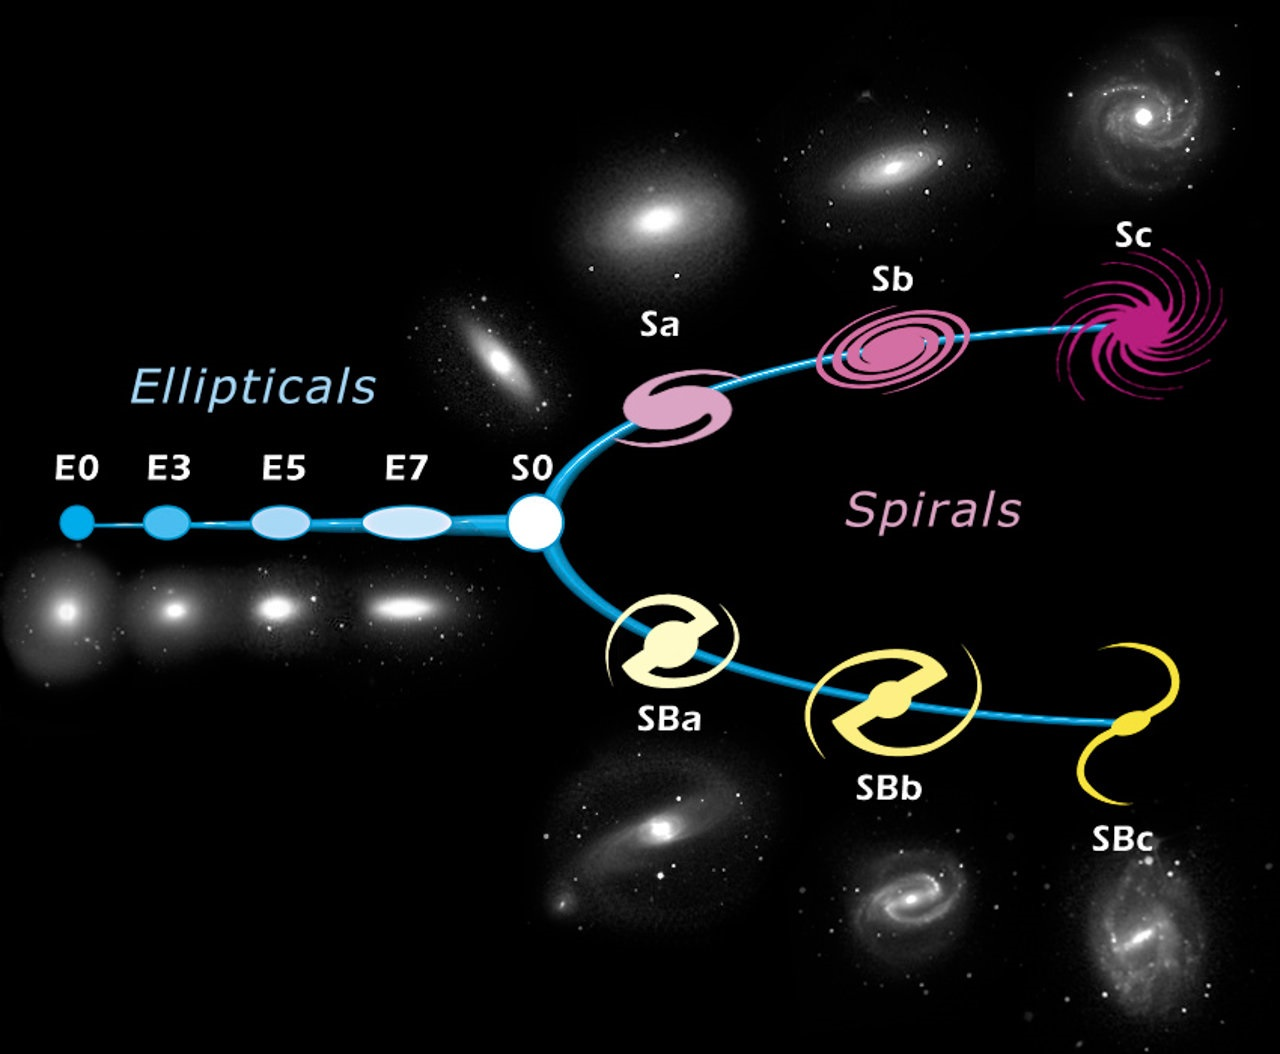
\includegraphics[width=\textwidth]{introduction/hubble.jpg}
	\caption[The Hubble tuning-fork]{The Hubble Diagram (or tuning fork) showing different optical image morphology classifications. Figure courtesy of http://spacetelescope.org}
	\label{fig:Hubble}
\end{figure}

\begin{figure}
	\centering
	% *********** Need to check permission for this figure *************
	% 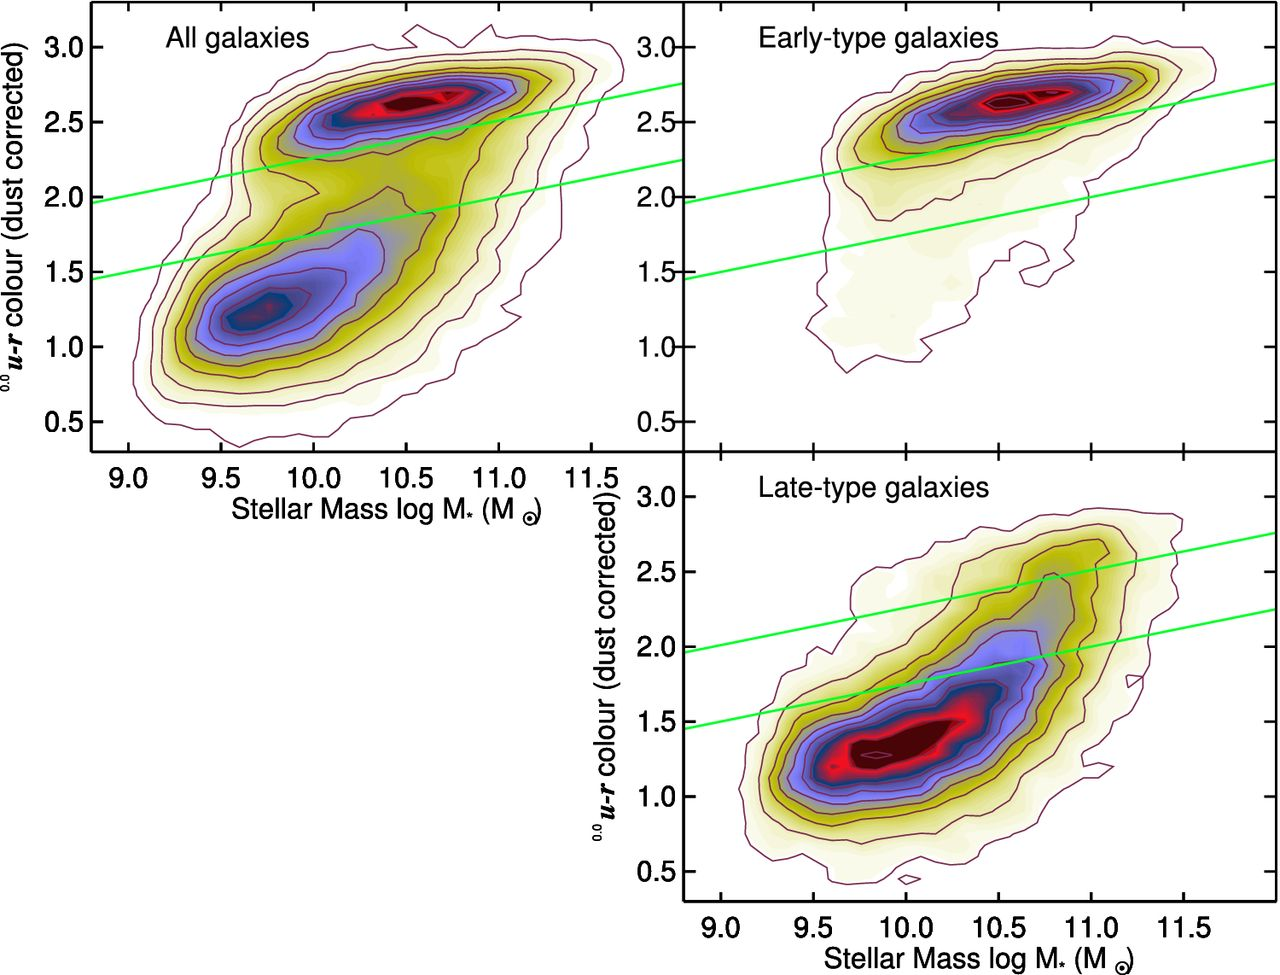
\includegraphics[width=\textwidth]{introduction/colorRedCorr_mass.jpeg}
	% \caption[Color--Mass diagram]{A reddening-corrected color--mass diagram showing the distribution of ETGs and LTGs on the color--mass plane with the red sequence, blue cloud and dividing green valley labeled. Figure courtesy of \citet{Schawinski2014}}
	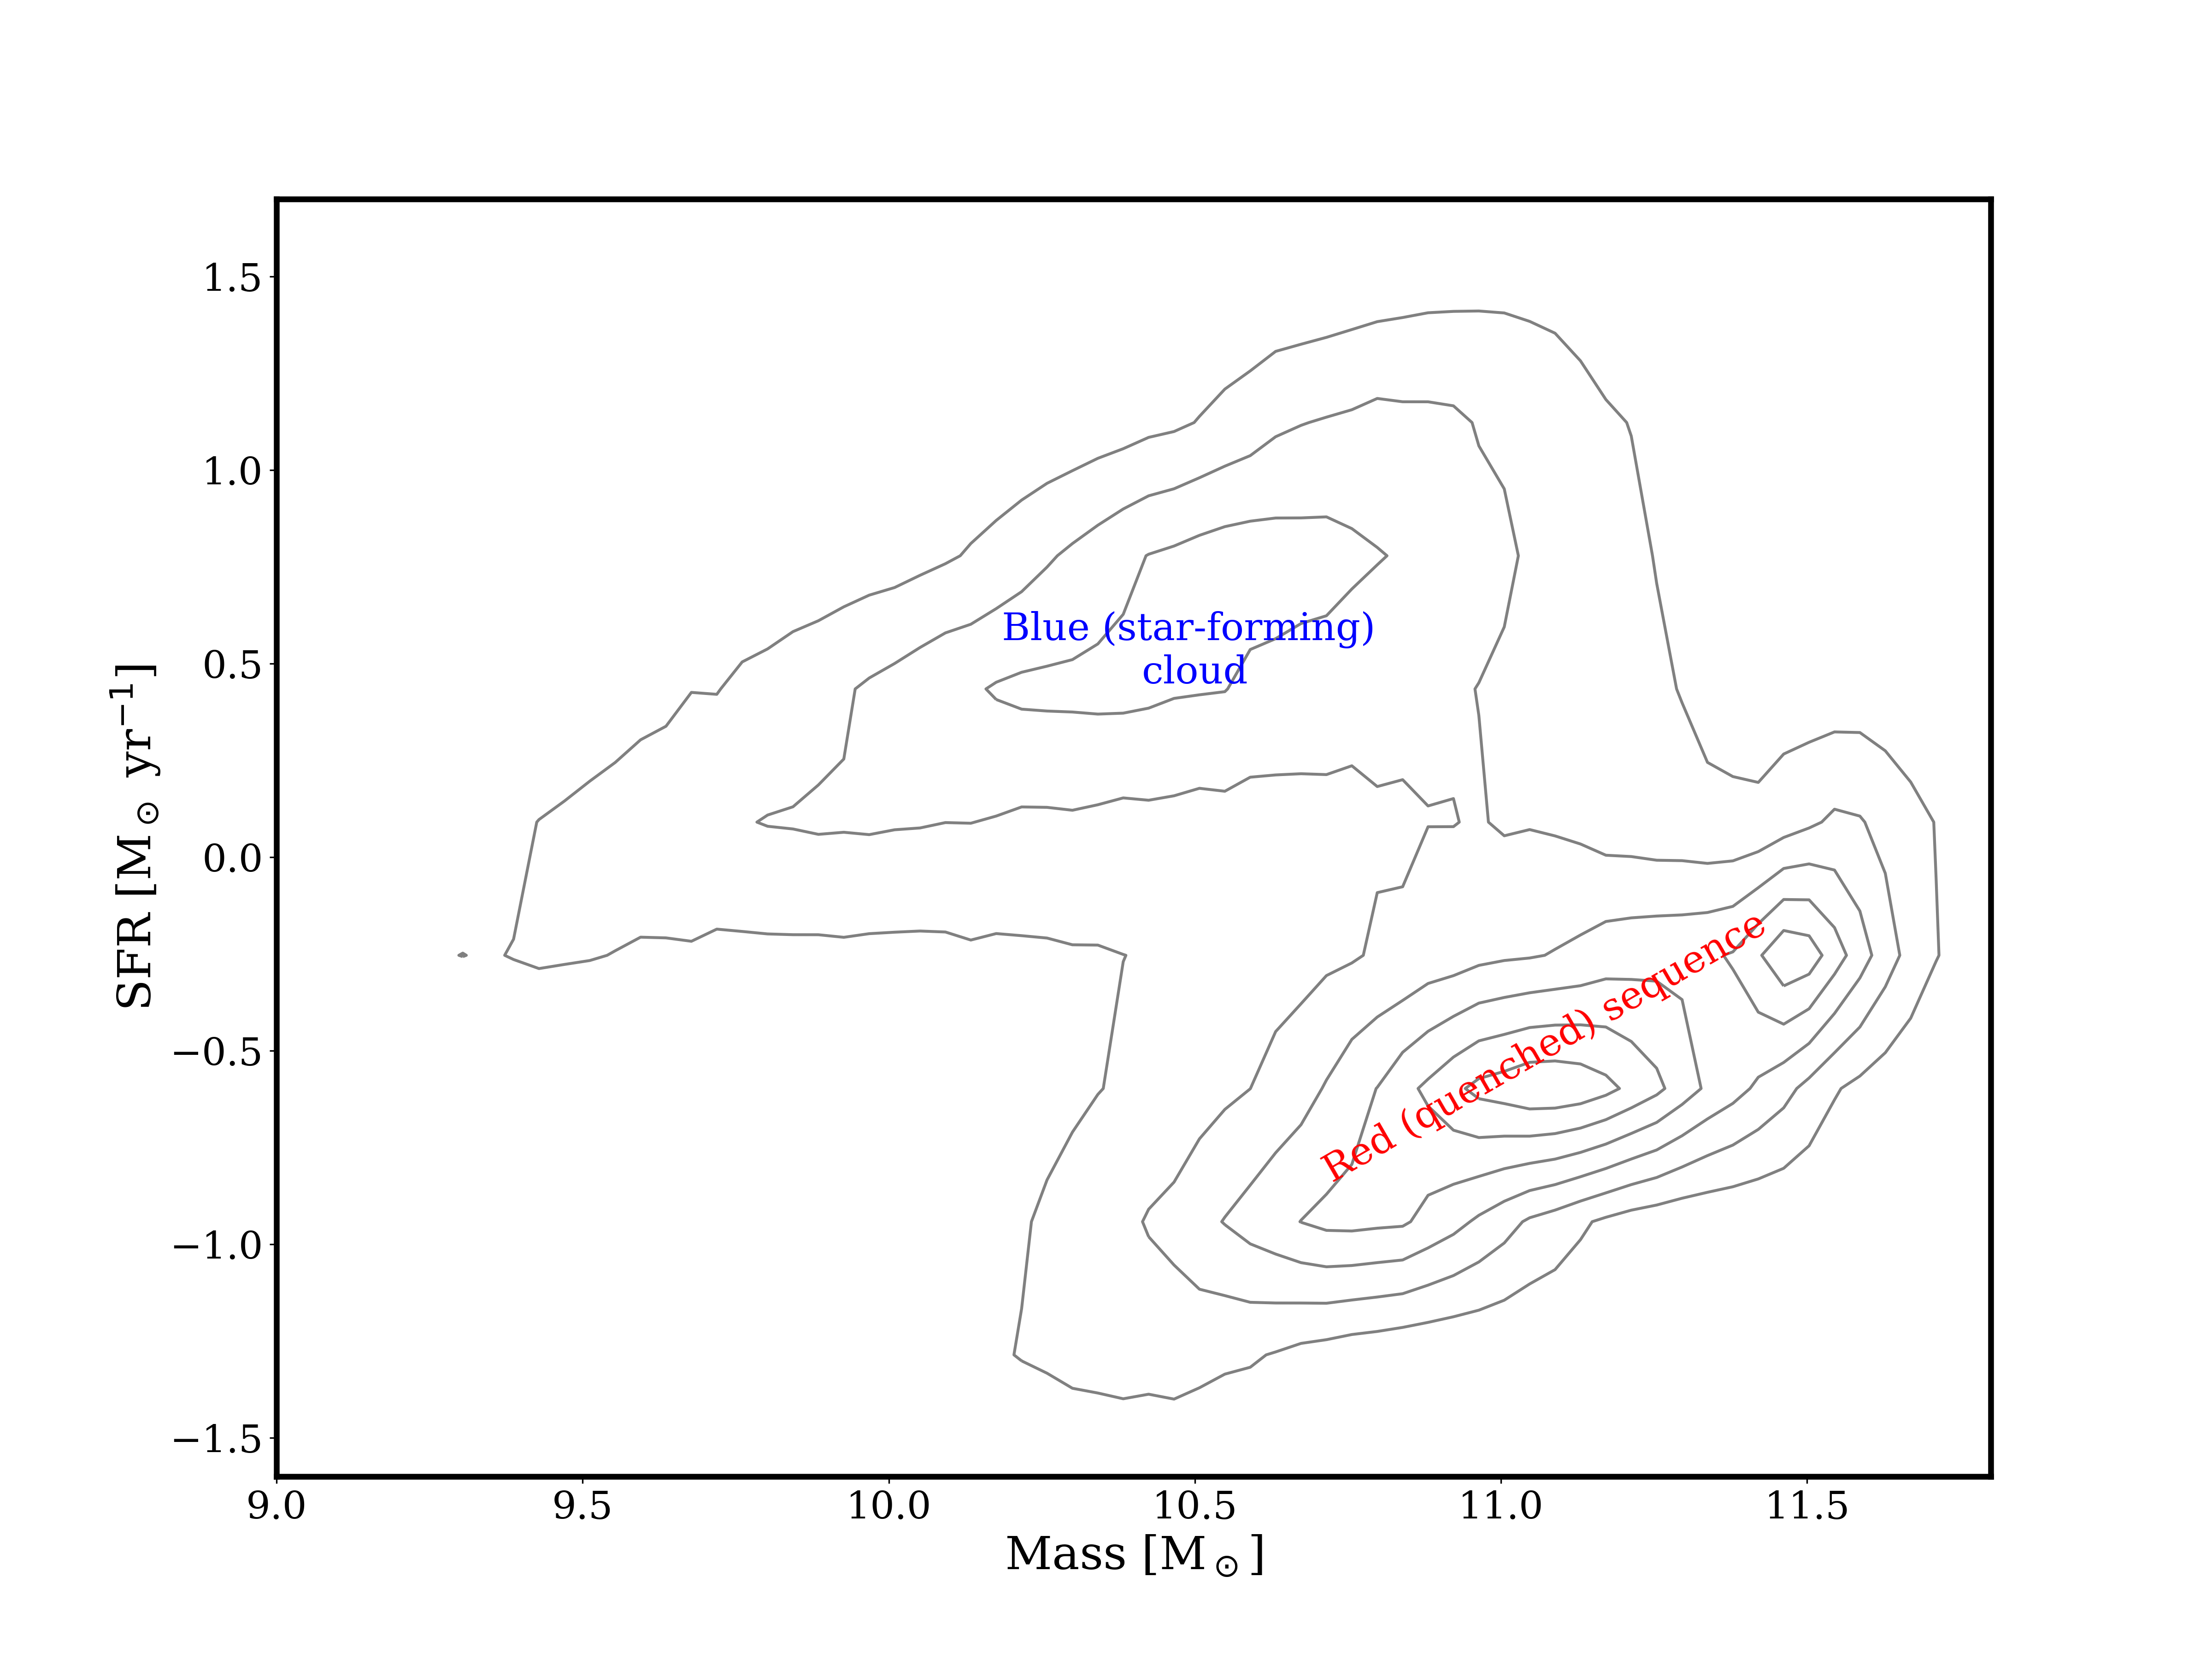
\includegraphics[width=\textwidth]{introduction/sfMass.png}
	\caption[Star-formation rate--Mass diagram]{The dichotomy in the star-formation rate--mass plane for the MPA-JHU sample (i.e. SDSS DR7) galaxies \citep{Kauffmann2003, Brinchmann2003, Salim2007}.}
	\label{fig:colorMass}
\end{figure}

Given their low star formation rates, ETGs are dominated by old stars, while spirals are dominated by young stars. The reasons for this dichotomy is a major part of modern astrophysics. ETGs are often the most massive galaxies, so they clearly must have undergone substantial star formation in their early history which has now stopped. They either must have run out of fuel for forming stars or have undergone (or have ongoing) some process which is preventing star formation. Many have been observed to contain large reservoirs of cold (molecular) gas \citep{}, the material from which stars are formed: this seems to favor the latter. The reservoirs are, however, significantly smaller than in LTGs.

Many studies now point to the fact that most (if not all) galaxies contain a super-massive black hole at the center \citep{Kormendy2013a}. They show that there are tight correlations (known as scaling relations) between the properties of the central black hole and the host galaxy despite orders of magnitude differences between the sphere of gravitational influence of the black hole and the size of the host galaxy \citep{Gudehus1973, Faber1976, Ferrarese2000, Gebhardt2000}. 

It is also seen that many galaxies contain a bright point source at the center. These are known as Active Galactic Nuclei (AGN) and in extreme cases these can completely outshine the combined starlight of the host galaxy (these extreme AGN are known as quasars). AGN are understood to be the result of accretion of the inter-stellar medium (ISM) onto the central black hole \citep{Lynden-Bell1969} and the energy emitted by the AGN is generally invoked to explain the scaling relationships \citep{Raimundo2010} as well as the quenching of star formation in ETGs \citep{Croton2006, Somerville2008}. This is known as AGN feedback and appears to be required by current numerical simulations and semi-analytic models to successfully reproduce the observed properties of massive galaxies \citep{Kauffmann2000, Granato2004, DiMatteo2005, Springel2005, Bower2006, Croton2006, Hopkins2006, Ciotti2010, Scannapieco2012}. The exact fraction of galaxies that contain AGN varies depending on the selection method for the AGN, but it strongly mass dependent, with more massive galaxies more likely to contain an AGN \citep{Kauffmann2003a}. 

AGNs are very varied, however much work has been done on a single unified model, where the differences between individual observations can be explained by differing orientations of the AGN. The Unified Model by \citet{Antonucci1993} describes AGN as made up of up to five components or regions surrounding the central black hole: (i) immediately around the black hole is an accretion disk. Surrounding this is (ii) a dust obscuring structure which is torus in shape. This blocks a side-on view of the black hole and accretion disk. Intense radiation from the accretion disk ionizes (iii) the region immediately above and below the disk. This emits in the optical regime with and due to the proximity to the black hole the gas has very high orbital velocities ($\sim 5000 \mathrm{km s^{-1}$) giving rise to its characteristic broad lines and the name: broad-line region (BLR). The BLR is also obscured by the torus if viewed edge-on. Beyond this is (iv) the narrow-line region (NLR), an area of more sedate velocities ($\sim 200 \mathrm{km s^{-1}$) and less ionized gas. Becuase of the shadow cast by the torus the NLR is sometimes seen in a cone shape \citep{Wilson1994}. Finally, a small proportion of AGN contain (v) jets of plasma traveling at relativistic speeds out from the poles of the accretion disk (the exact orientation of the jet may well also be dependent of the orientation of the spin of the black hole, though this remains an unknown). The nature of the jet is explored in more detail below. AGN viewed side-on, with the black hole, accretion disk and BLR obscured by the torus are known as Type 2 AGN, while AGN viewed face-on, sometime viewing directly down the jet, are known as Type 1. A schematic the unified model is shown in figure \ref{fig:UnifiedAGN}

% Permission given without request for using in a thesis
\begin{figure}
	\centering
	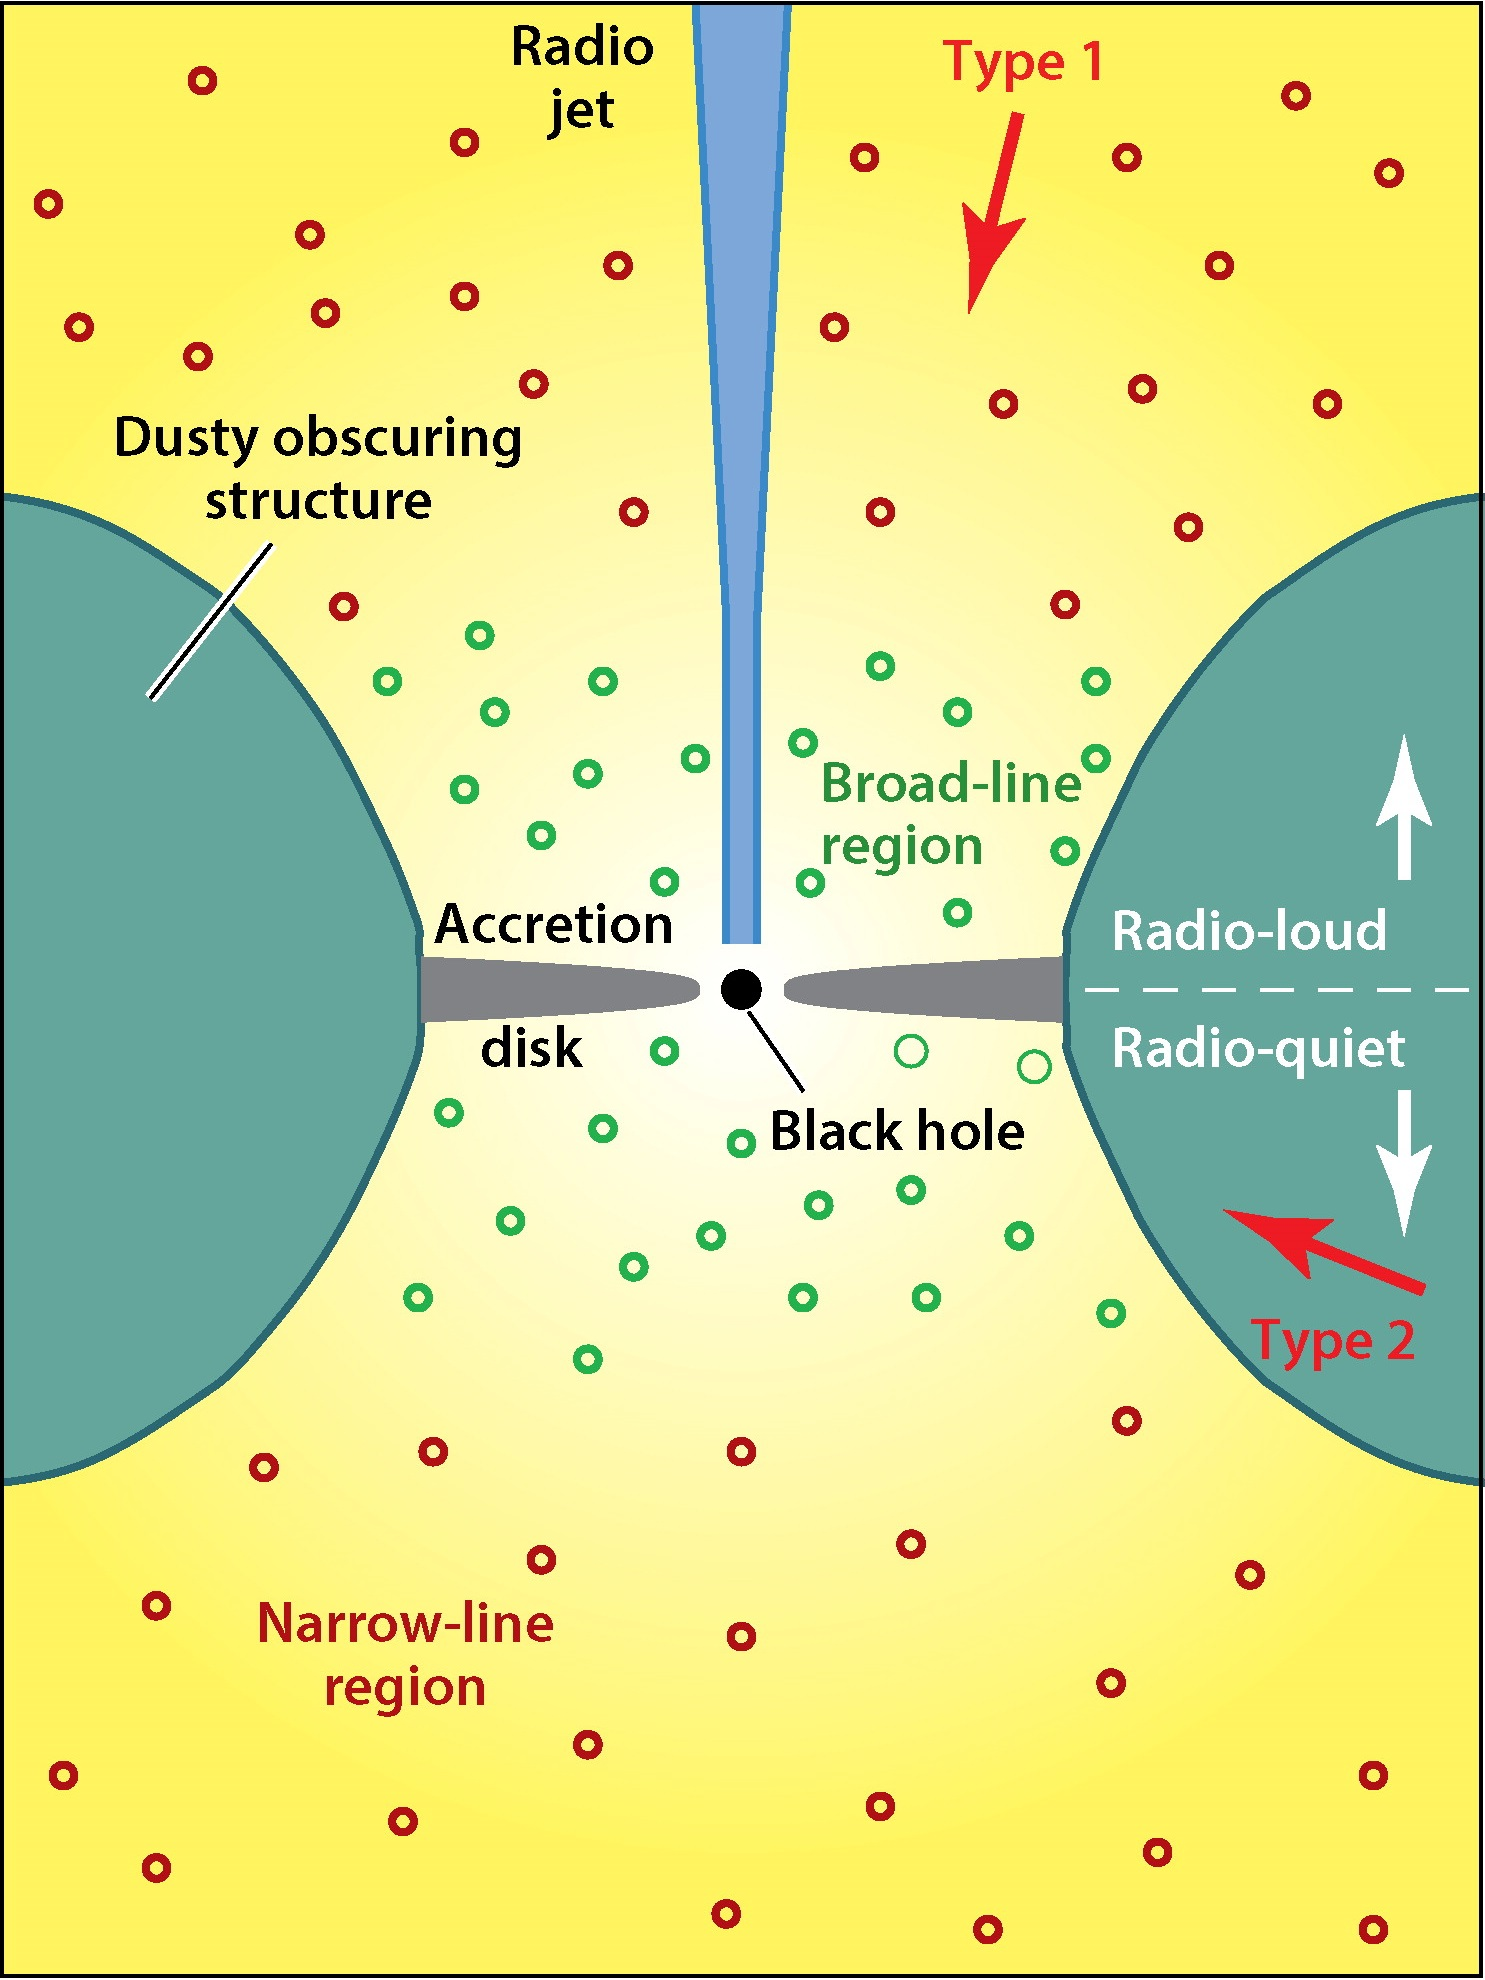
\includegraphics[width=\textwidth]{introduction/unifiedAGN.jpeg}
	\caption[Schematic of unified model of AGN]{A schematic of the unified model of AGN. The primary source of radiation is the accretion disk. This in tern ionizes both the broad-line and the narrow-line regions. A dust torus obscures a side-on view (Type 2 AGN), while a jet sometimes occurs from the poles of the disk. Figure courtesy of \citet{Heckman2014}}
	\label{fig:UnifiedAGN}
\end{figure}

Despite the unification of the many observed morphologies of AGN, it is becoming increasingly clear that AGNs do exist in two different modes, Radiative and Jet-mode \citep{Antonucci2012}, raising speculation about differing mechanisms and possibly fuel sources for each. More detail on both modes can be found in section \ref{sec:AGN}. 

Although all galaxies emit at some level in all frequencies, only some emit in the radio at a detectable (with current instrumentation) levels and even then most are extremely faint. These galaxies are known as radio galaxies (RGs) and most radio emission is attributed to synchrotron emission (the broader term of free-free emission is sometimes used in the literature) from the jet within an AGN. However, \citet{Nyland2016} notes that in the fainter sources, the radio emission could be consistent with circumnuclear star formation. There is broad consensus within the literature that the most powerful RGs are the product of gas rich (wet), major mergers of galaxies (a major merger is defined as a ratio in mass closer than 3:1 between progenitor galaxies). These AGN tend to be extremely luminous: indeed despite clearly containing a very powerful jet, they are mostly radiative mode AGN. These RGs form a very small minority of the RG population and hence are not representative. \citet{Heckman2014} presents evidence that most RGs are fueled through secular processes. Exploring the nature and origin of the fuel, as well as the mechanism of accretion and effect of the resulting AGN feedback in RGs forms the basis of this thesis. 

The rest of this chapter will cover the background required to study the RG population. Firstly, since RGs are mostly found in ETGs we will cover our current understanding of ETGs. This is mostly a summary of the recent Integral Field Spectroscopy (IFS) surveys including Atlas3D, MaNGa, MASSIVE, SAMI and Califa and can be considered a setting out of the control sample for our later investigations. After this we will give a more detailed summary of the current state of our understanding of AGN. This will include covering RGs. Finally we will set out our selection criteria and sample which we use to acheive our aim of understanding the feeding and feedback of RGs.

\section{Early Type Galaxies}
	\label{sec:ETG}
	In this section we mostly summarize Cappellari's excellent review of IFS studies of ETGs \citep{Cappellari2016}. 

	Confusingly, due to historical reasons there are several, similar, yet subtly different definitions for the LTG/ETG classes. Originally they were based purely on the morphology as seen in optical images: spirals were LTGs and ellipticals were ETGs, while there was ongoing debate about which class to place lenticular galaxies (S0s). S0s appeared disk-like like LTGs, but were often seen to contain older populations with less star-formation like ETGs. This debate has confused the literature, with some taking the classification scheme to reflect the underlying stellar population and others the assumed method of support (rotational or dispersion). In this thesis we use the stellar population view and such would include S0s within the ETG class.

	One useful morphological classification within ETGs is the nuclear surface brightness profile. It was noted that some galaxies showed significant flattening of the surface brightness profile towards the center of the galaxy (cored galaxies), whereas others only showed only mild changes (power-law galaxies). An example of each is shown in figure \ref{fig:CorePower} for galaxies NGC 596 and NGC 1399. This is parameterized using a double power-law of the form:
	\begin{align}
		\Sigma(R) = & \Sigma_b \left(\frac{R_b}{R}\right)^\gamma \left[\frac{1}{2} + \frac{1}{2}\left(\frac{R}{R_b}\right)^\alpha\right]^{\frac{\gamma-\beta}{\alpha}}
		\label{eq:Nuker} \\
		\intertext{where $\gamma$ and $\beta$ control the inner and outer slope respectively, $R_b$ is the position of the transition between inner and out slopes, $\Sigma_b$ is the surface brightness at $R_b$ and $\alpha$ sets the speed of transition. A galaxy is classifed using the derivative $\gamma'$:}
		\gamma' \equiv & - \frac{\mathrm{d}\log I}{\mathrm{d} \log R} \right|_{R=R'} = - \frac{\gamma + \beta \left(\frac{R'}{R_b}\right)^\alpha}{1 + \left(\frac{R'}{R_b}\right)^\alpha}
	\end{align}
	at Hubble Space Telescope (HST) resolution limit of $R' = 0.1 \, \text{arcsec}$. If $\gamma' \le 0.3$ is a considered a cored galaxy, while $\gamma' \ge 0.5$ is called a power-law (or 'cuspy') galaxy. In the range $0.3 < \gamma' < 0.5$, galaxies are considered intermediate. High resolution images have shown that in 2D images, cored galaxies have 'boxy' isophotes, while power-law galaxies have 'disky' isophotes \citep{Lauer1995, Faber1997}. Further more, these respectively correspond to triaxial and oblate 3D shapes.

	\begin{figure}
		\centering
		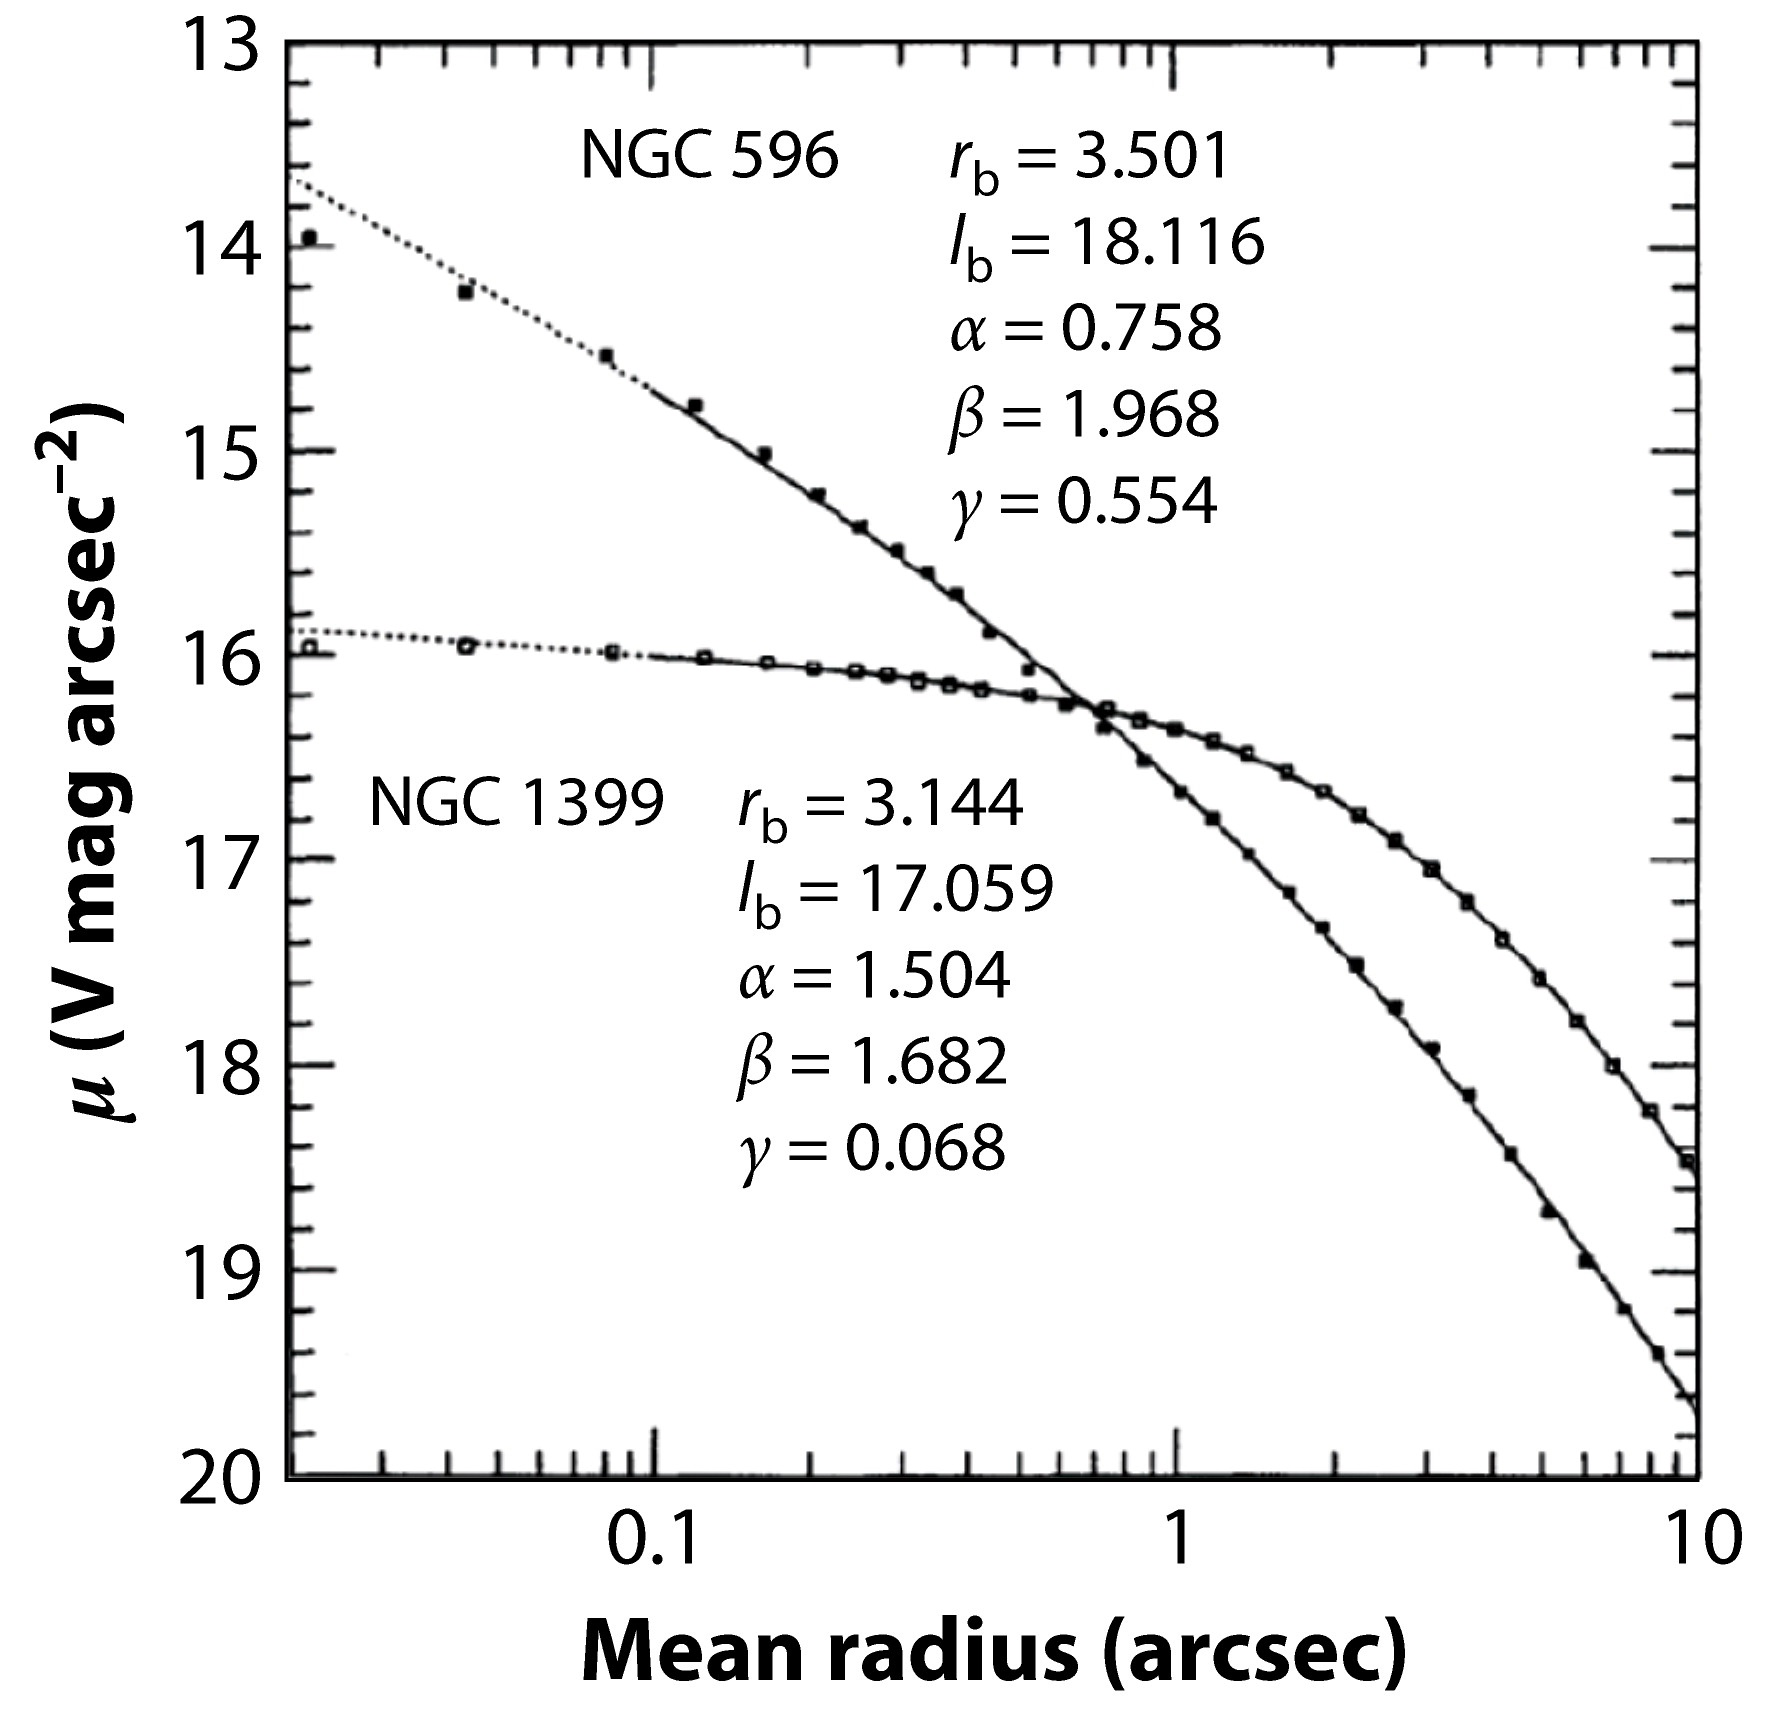
\includegraphics[width=\textwidth]{introduction/exampleCorePower.jpeg}
		\caption[Example cored and power-law surface brightness profile]{Two example galaxies: NGC 596 and NGC 1399 which display a power-law and cored morphology respectively. Both are fitted with the double power law (eq. \ref{eq:Nuker}) shown with the black line. Both galaxies have similar outer slopes, but dramatically different inner slopes. Figure courtesy of \citet{Lauer1995}}
		\label{fig:CorePower}
	\end{figure}

	The Atlas3D survey \citep{Cappellari2011} found that morphologically categorizing ETGs into ellipticals and S0s was misleading and did not reflect any physical background. Instead they used spatially resolved kinematics to classify ETGs into fast (rotationally supported) or slow (dispersion supported) rotators, depending on their value of $\lambda_R$ \citep{Emsellem2011}. $\lambda_R$ is a new parameter that reflects the galaxies specific angular momentum and is defined as:
	%Change this to other definitions
	\begin{equation}
		\lambda_R \equiv \frac{\langle R |V_\ast|\rangle}{\langle R \sqrt{V_\ast^2 + \sigma_\ast^2}\rangle}
	\end{equation}
	where the angled the angled brackets represent the flux weighted average within a radius, $R$, $V_\ast$ is the is the stellar velocity and $\sigma_\ast$ is the stellar velocity dispersion for a given spatial bin. The most recent definition for if a galaxy is considered a slow rotator is:
	\begin{equation}
		\lambda_{R_e} < 0.08 + \frac{\epsilon}{4} \text{  and  } \epsilon < 0.4
	\end{equation}
	where $\epsilon$ is the ellipticity and $\lambda_{R_e}$ the value of $\lambda_R$ evaluated at the effective radius ($R_e$) \citep{}. % Need to find original place this was defined (not just Michele's review).
	It is worth noting here that while most S0s are fast rotators and most slow rotators are ellipticals, the counter arguments are not necessarily true: many ellipticals are fast rotators and not all fast rotators are S0s. In fact the dichotomy is better reflected by the core verse power-law morphologies, though \citet{Cappellari2016} notes that the kinematic classification scheme has the advantage that it is nearly inclination independent and can be measured at much lower spatial resolutions. Having said that, the cases where they do not agree are often pointers to misclassified kinematics, such as counter rotating disks that have been erroneously classified as a slow rotator \citep{Pinkney2003, Cappellari2005, Cappellari2007}. 

	It was found that most slow rotators are massive, with $M \gtrsim 10^{10.5} M_\odot$ and that they dominate the high mass end, though fast rotators dominate by a factor of $\sim 7$ in overall numbers \citep{Emsellem2011, Veale2016}. Figure \ref{fig:SlowRotFrac} shows the change in proportion of slow rotators as a function of stellar mass (for which K-band magnitude, $M_K$, is used as a proxy).


	\begin{figure}
		\centering
		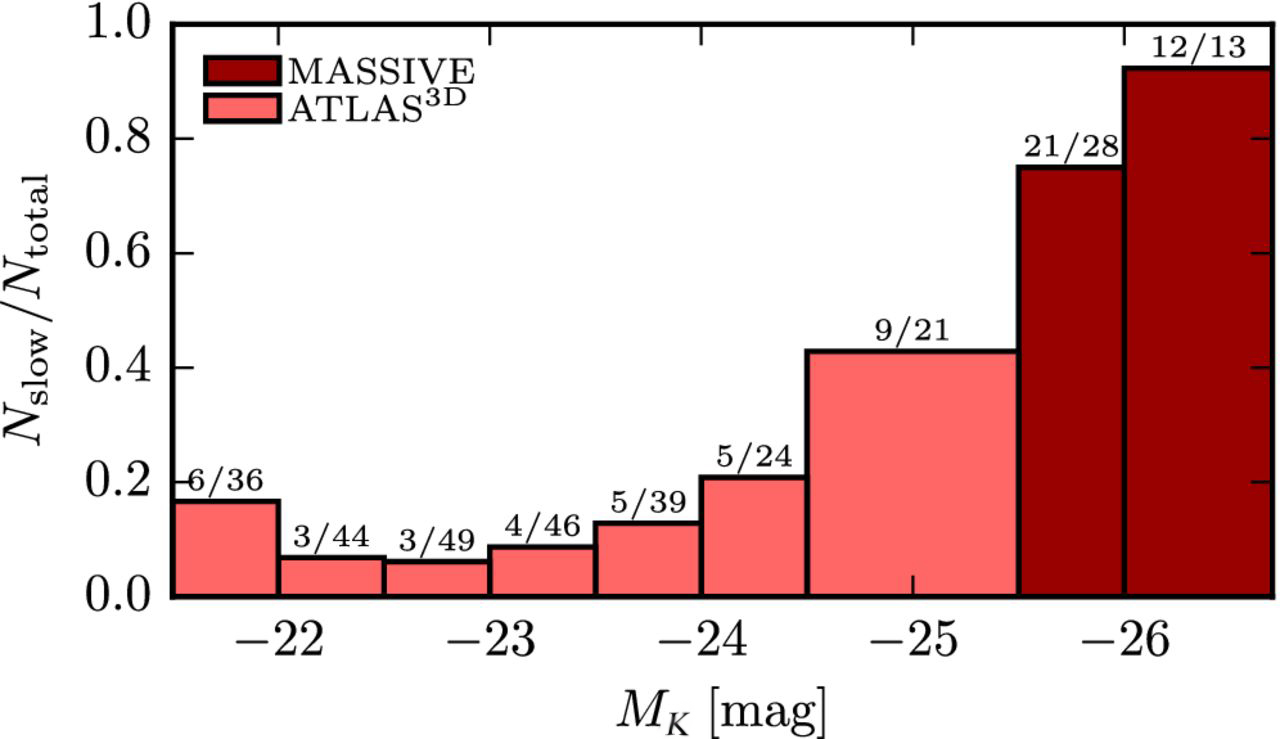
\includegraphics[width=\textwidth]{introduction/slowRotFraction.jpeg}
		\caption[Proportion of Slow Rotating Galaxies as a function of Mass]{The fraction of slow rotators within the total number of galaxies within a given K-band magnitude ($M_K$). $M_K$ is used here as a proxy for stellar mass. Figure courtesy of \citet{Veale2016}}
		\label{fig:SlowRotFrac}
	\end{figure}

	Fast rotators were found to reflect many proprieties of and have strikingly similar distributions to spirals. Fast rotators can be shown to contain disks, even very round objects can be shown to be face-on disks \citep{Cappellari2013a, Weijmans2014}. They also have very similar bulge fraction range \citep{Krajnovic2013} and clustering distributions \citep{}. % is this true? Fig 25 in Michele's review shows very different morphology density relation for FR vs spirals.
	In figure \ref{fig:MassRe} fast rotators form a parallel series to spiral galaxies.

	The discovery of the fast/slow rotator scheme re-ignites the S0 debate and lead the Atlas3D group to re-evaluate the Hubble sequence: they proposed the Atlas3D comb (shown in figure \ref{fig:Atlas3Dcomb}) \citep{Cappellari2011a}, where the evolution path of a typical galaxy is from disk to bulge dominated is along one of the fingers of the comb. If the disk is destroyed the galaxy then evolves down the handle of the comb, becoming a slow rotator. 

	\begin{figure}
		\centering
		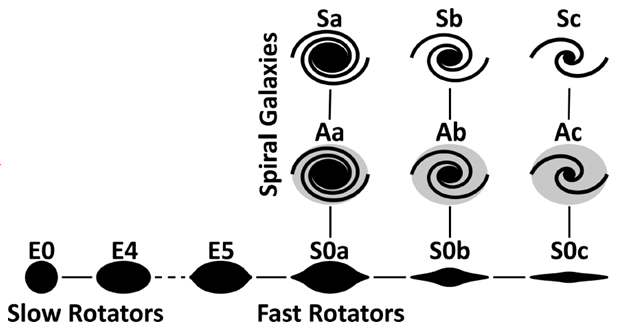
\includegraphics[width=\textwidth]{introduction/Atlas3D_comb.png}
		\caption[The Atlas3D comb]{The Atlas3D comb, a replacement to the Hubble tuning fork (fig \ref{fig:Hubble}). Figure courtesy of \citet{Cappellari2011a}}
		\label{fig:Atlas3Dcomb}
	\end{figure}

	Since \citet{Sarzi2015} has shown an inner power-law has been shown to be fragile to dry major mergers, cored galaxies are assumed to be markers that the galaxy has undergone such a merger. The near 1:1 correspondence between slow/fast rotators and cored/power-law classification schemes shows that this must also be responsible for forming slow rotators and changing the shape of the galaxy from oblate to triaxial.

	One useful test for a triaxial shape is misalignment between the kinematic rotation axis and the apparent minor axis. For oblate structures these should align within $\sim 5$\textdegree, however for triaxial structures they can have any orientation \citep{Contopoulos1956, Stark1977, Statler1987}. 

	\begin{figure}
		\centering
		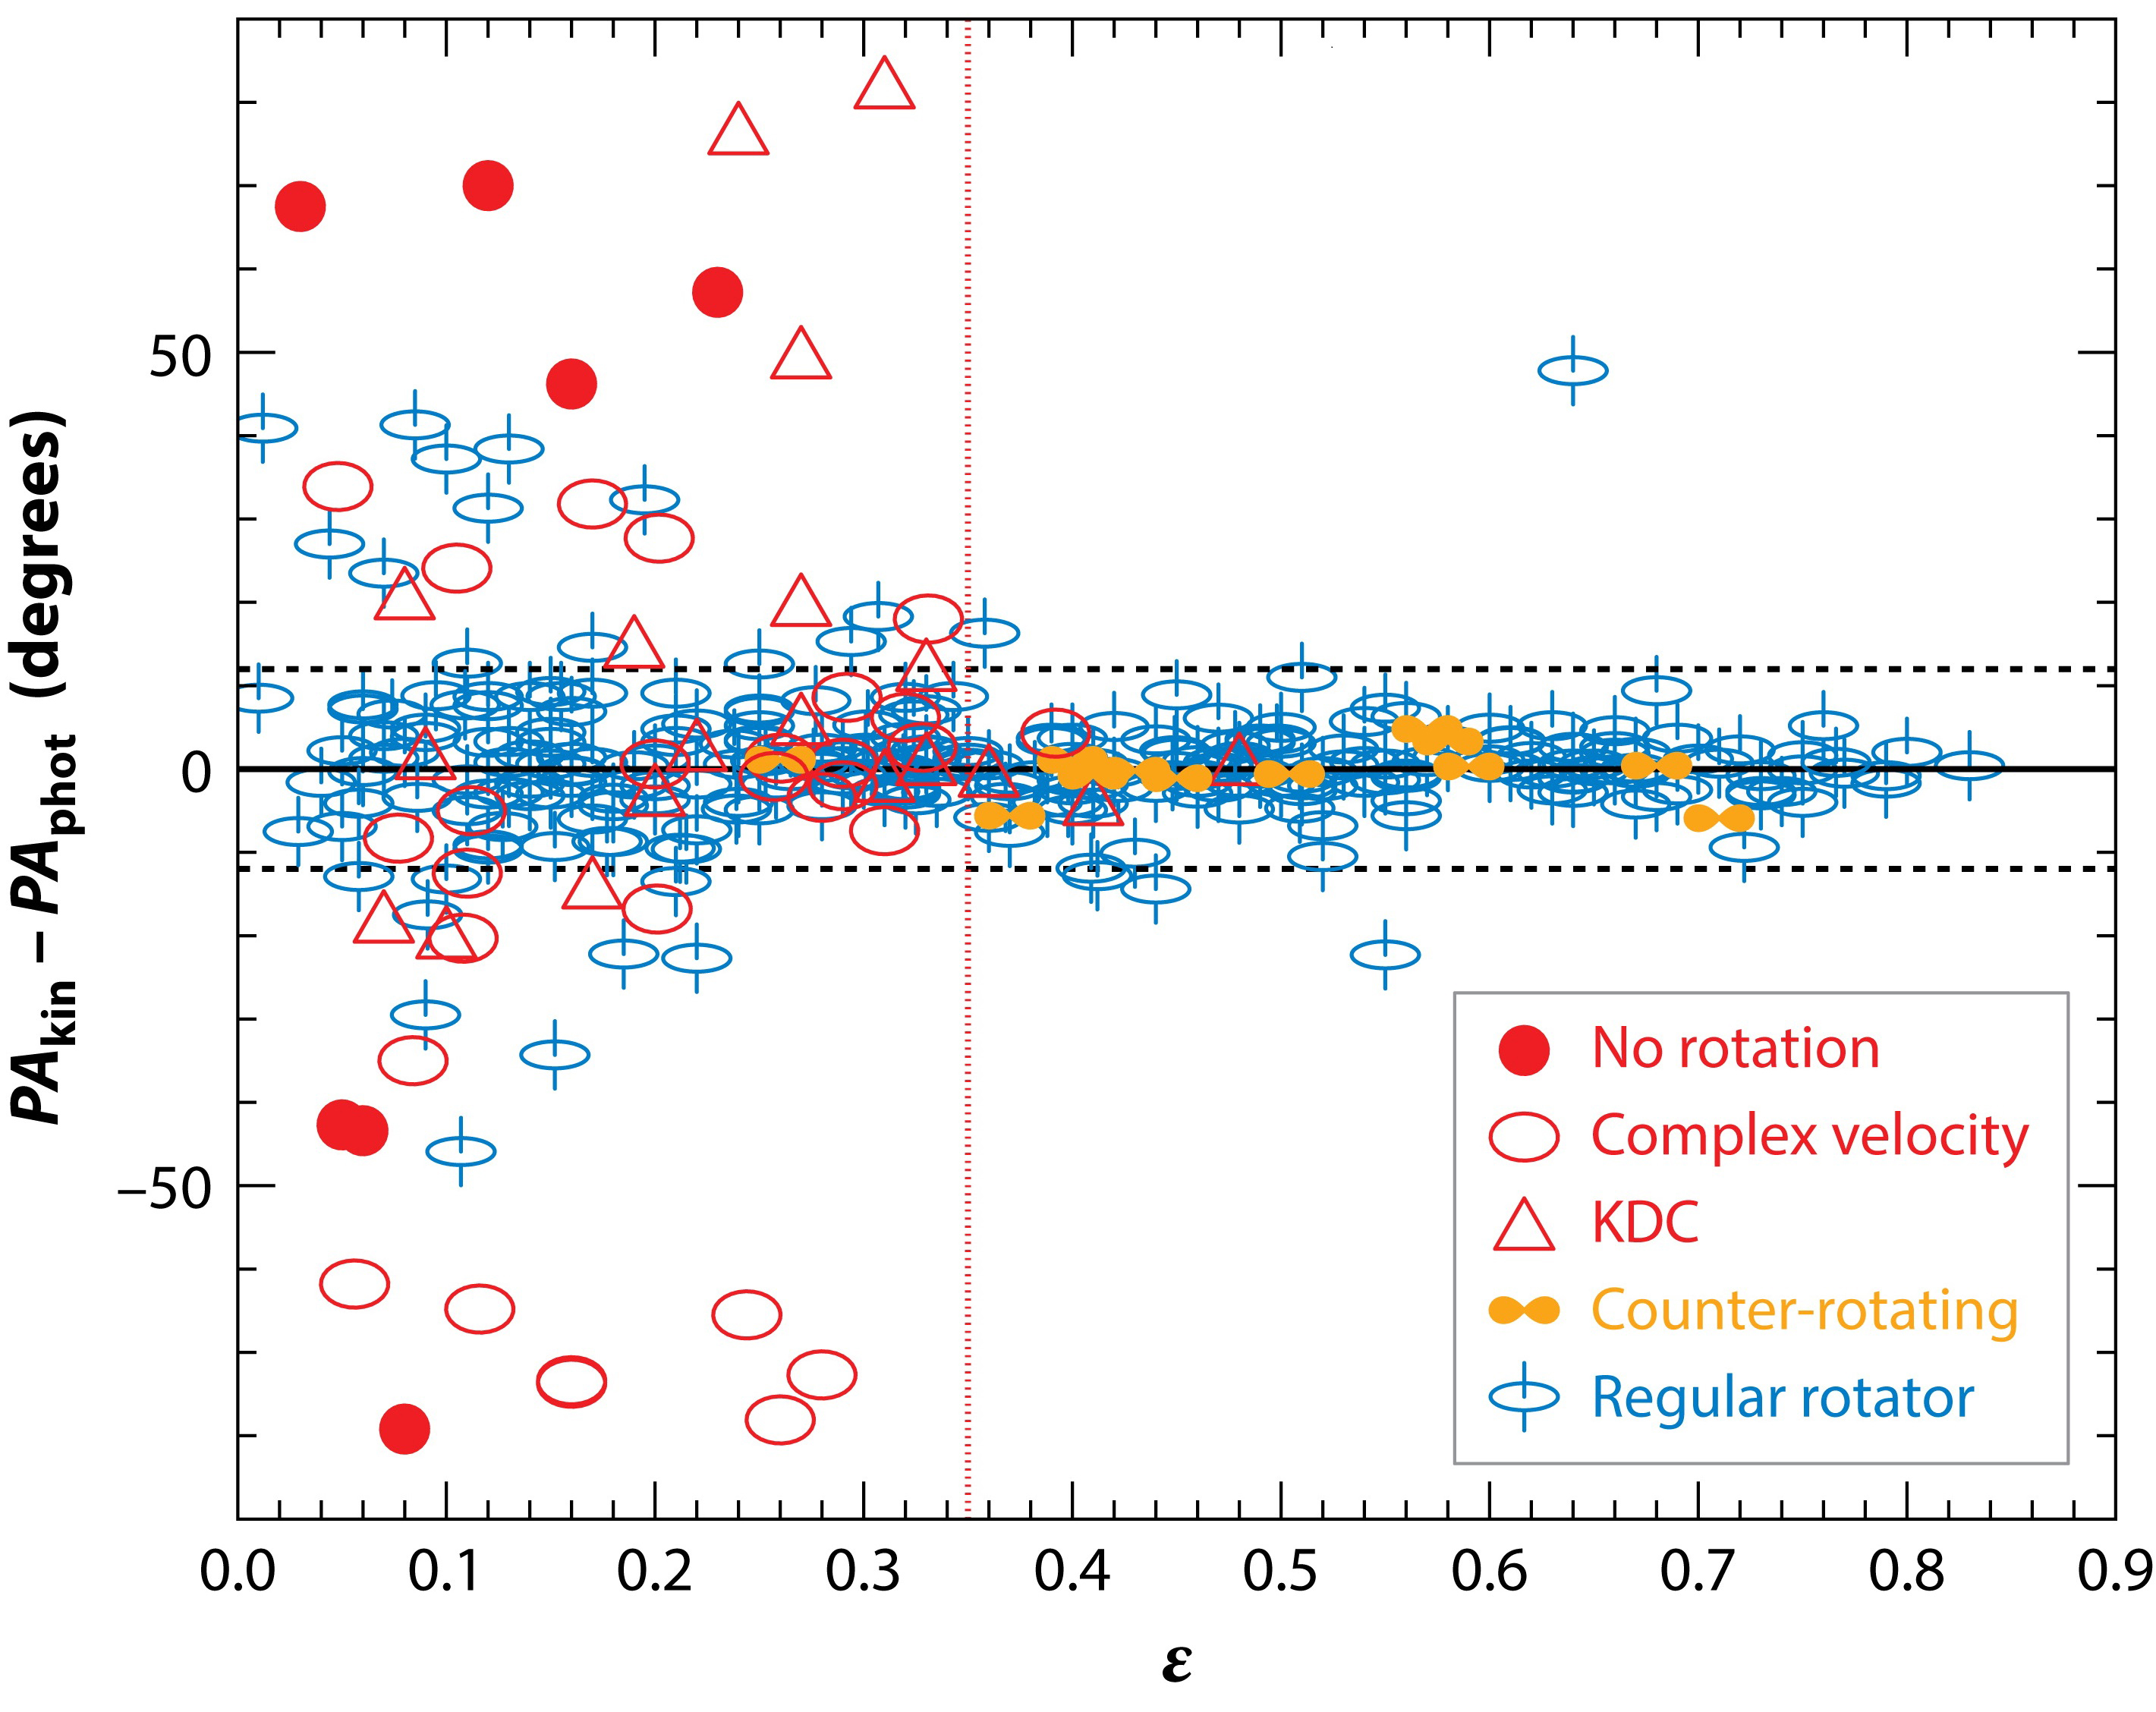
\includegraphics[width=\textwidth]{introduction/misalignment.jpg}
		\caption[The kinematic--photometric misalignment in slow rotators]{This figure shows the misalignment of the position angles (PA) of non-regularly rotating galaxies for Atlas3D and SAMI pilot study galaxies. Slow rotators are defined for ellipticity, $\epsilon$, $<0.3$. Figure courtesy of \citet{Cappellari2016}. KDC is an abbreviation of kinematically decoupled cores.}
		\label{fig:MassRe}
	\end{figure}

	In figure \ref{fig:MassRe} we can see Atlas3D comb structure in the physically meaningful mass--size plane. Galaxies evolve along lines of constant angular momentum (upper, left to lower center) through gas accretion onto the bulge. A major, dry merger then evolves the galaxy into a slow rotator \citep{Bendo2000} with similar properties to those observed by Atlas3D \citep{Jesseit2007, Jesseit2009}, where the bulk of added mass is from continuous minor mergers \cite{DeLucia2007, Genel2008, Feldmann2010, Oser2010, Feldmann2011, Hirschmann2012}. This moves the galaxy from lower center to upper right in figure \ref{fig:MassRe}. 

	\begin{figure}
		\centering
		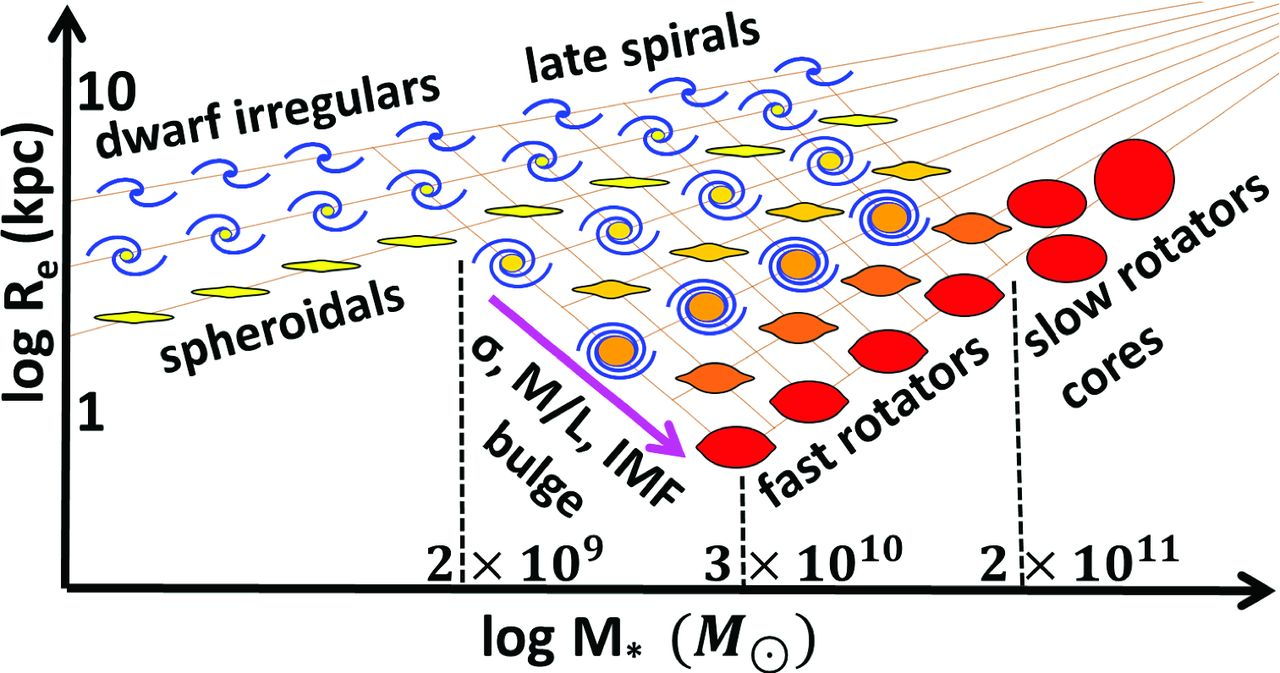
\includegraphics[width=\textwidth]{introduction/mass_Re.jpg}
		\caption[The galaxy mass--size plane]{This figure clearly shows the Atlas3D comb structure when dwarf galaxies are neglected. Figure courtesy of \citet{Cappellari2013a}}
		\label{fig:MassRe}
	\end{figure}

	Atlas3D also found a raft of kinematic substructures or features. These were split into five categories, a-e, (examples shown in figure \ref{fig:EgSubstructure}) with a sixth category, f, containing unclassifiable objects \citep{Krajnovic2011}. These are mostly based on the analysis from the \textsc{kinemetry} routine\footnote{The IDL \textsc{kinemetry} routine is available from http://davor.krajnovic.org/idl/}. This parametrizes the velocity map by $V = V_\text{rot} \cos \theta$. The best-fitting ellipse is determined by minimizing all Fourier coefficients up the 3rd coefficient, $k_3$, except for the cosine term. Deviations from the cosine law are then represented by the $k_5$ harmonic \citep{Krajnovic2006}. Regular Rotators (RR, or galaxies that are well described by the cosine law) are defined as $\langle k_5/k_1 \rangle < 0.04$, which was based on the mean uncertainty of $k_5/k_1 \sim 0.03$ for all galaxies. All other galaxies are classed as non-regular rotators (NRR). Note that while RR/NRR classification broadly reflect fast/slow rotator classification, they should not be taken to have the same meaning. 

	Various kinematic features were also observed within the sample \citep{Krajnovic2011}. Galaxies are flagged as having:
	\begin{itemize}
		\item \textbf{No Features (NF)} if position angle of the best-fitting ellipse, $\mathrm{PA_kin}$, is constant with radius.
		\item \textbf{Double Maxima (2M)} morphology where the radial profile of $k_1$ rises to a local maximum followed by a fall and subsequent rise again. The outer maxima is usually larger than the inner one. 
		\item \textbf{Kinematic Twist (KT)} where $\mathrm{PA_kin}$ varies smoothly with an amplitude of at least 10\textdegrees. 
		\item \textbf{Kinematically Decoupled/Distinct Core (KDC)} if there is an abrupt change in $\mathrm{PA_kin}$ by more than 30\textdegree and $k_1$ drops to near zero in the transition region. \textbf{Counter-Rotating Cores (CRC)} are a special case where the change in $\mathrm{PA_kin}$ is about 180\textdegree.
		\item \textbf{Low Velocities (VL)} if $k_1 < 5 \mathrm{km s^{-1}}$. This below the threshold of the ability of \textsc{kinemetry} to establish the elliptical parameters. These galaxies can be considered non-rotating.
		\item \textbf{Double \textsigma (2\textsigma)} morphology if there are two off center, but symmetric peaks in the velocity dispersion. These galaxies are understood to contain two counter-rotating disks. 
	\end{itemize}
	Examples of each of the features above can be seen in figure 1 of \citet{Krajnovic2011}. The matching of these features with substructure categories is given in table \ref{tab:KinGroups}, which also lists the number of galaxies in which are flagged with each category in the Atlas3D sample. 

	\begin{table}
		\centering
		\caption{Kinematic Groups from Atlas3D (Col. 1), the number of galaxies from the Atlas3D sample out of 260 (Col. 2) and the kinematic features contained within the class (Col. 3). Table is reproduced from \citep{Krajnovic2011}}
		\label{tab:KinGroups}
		\begin{tabular}{c l l}
			\hline
			\hline
			Group 	& N$_{gals}	& Features \\
			\hline
			a 		& 7			& NRR/LV \\
			b 		& 12		& NRR/NF \\
			c 		& 19		& NRR/KDC, NRR/CRC, RR/CRC \\
			d 		& 11		& NRR/2\textsigma, RR/2\textsigma \\
			e 		& 209		& RR/NF, RR/2M, RR/KT \\
			f 		& 2			& Unclassified \\
			\hline
			\hline
		\end{tabular}
	\end{table}

	\begin{figure}
		\centering
		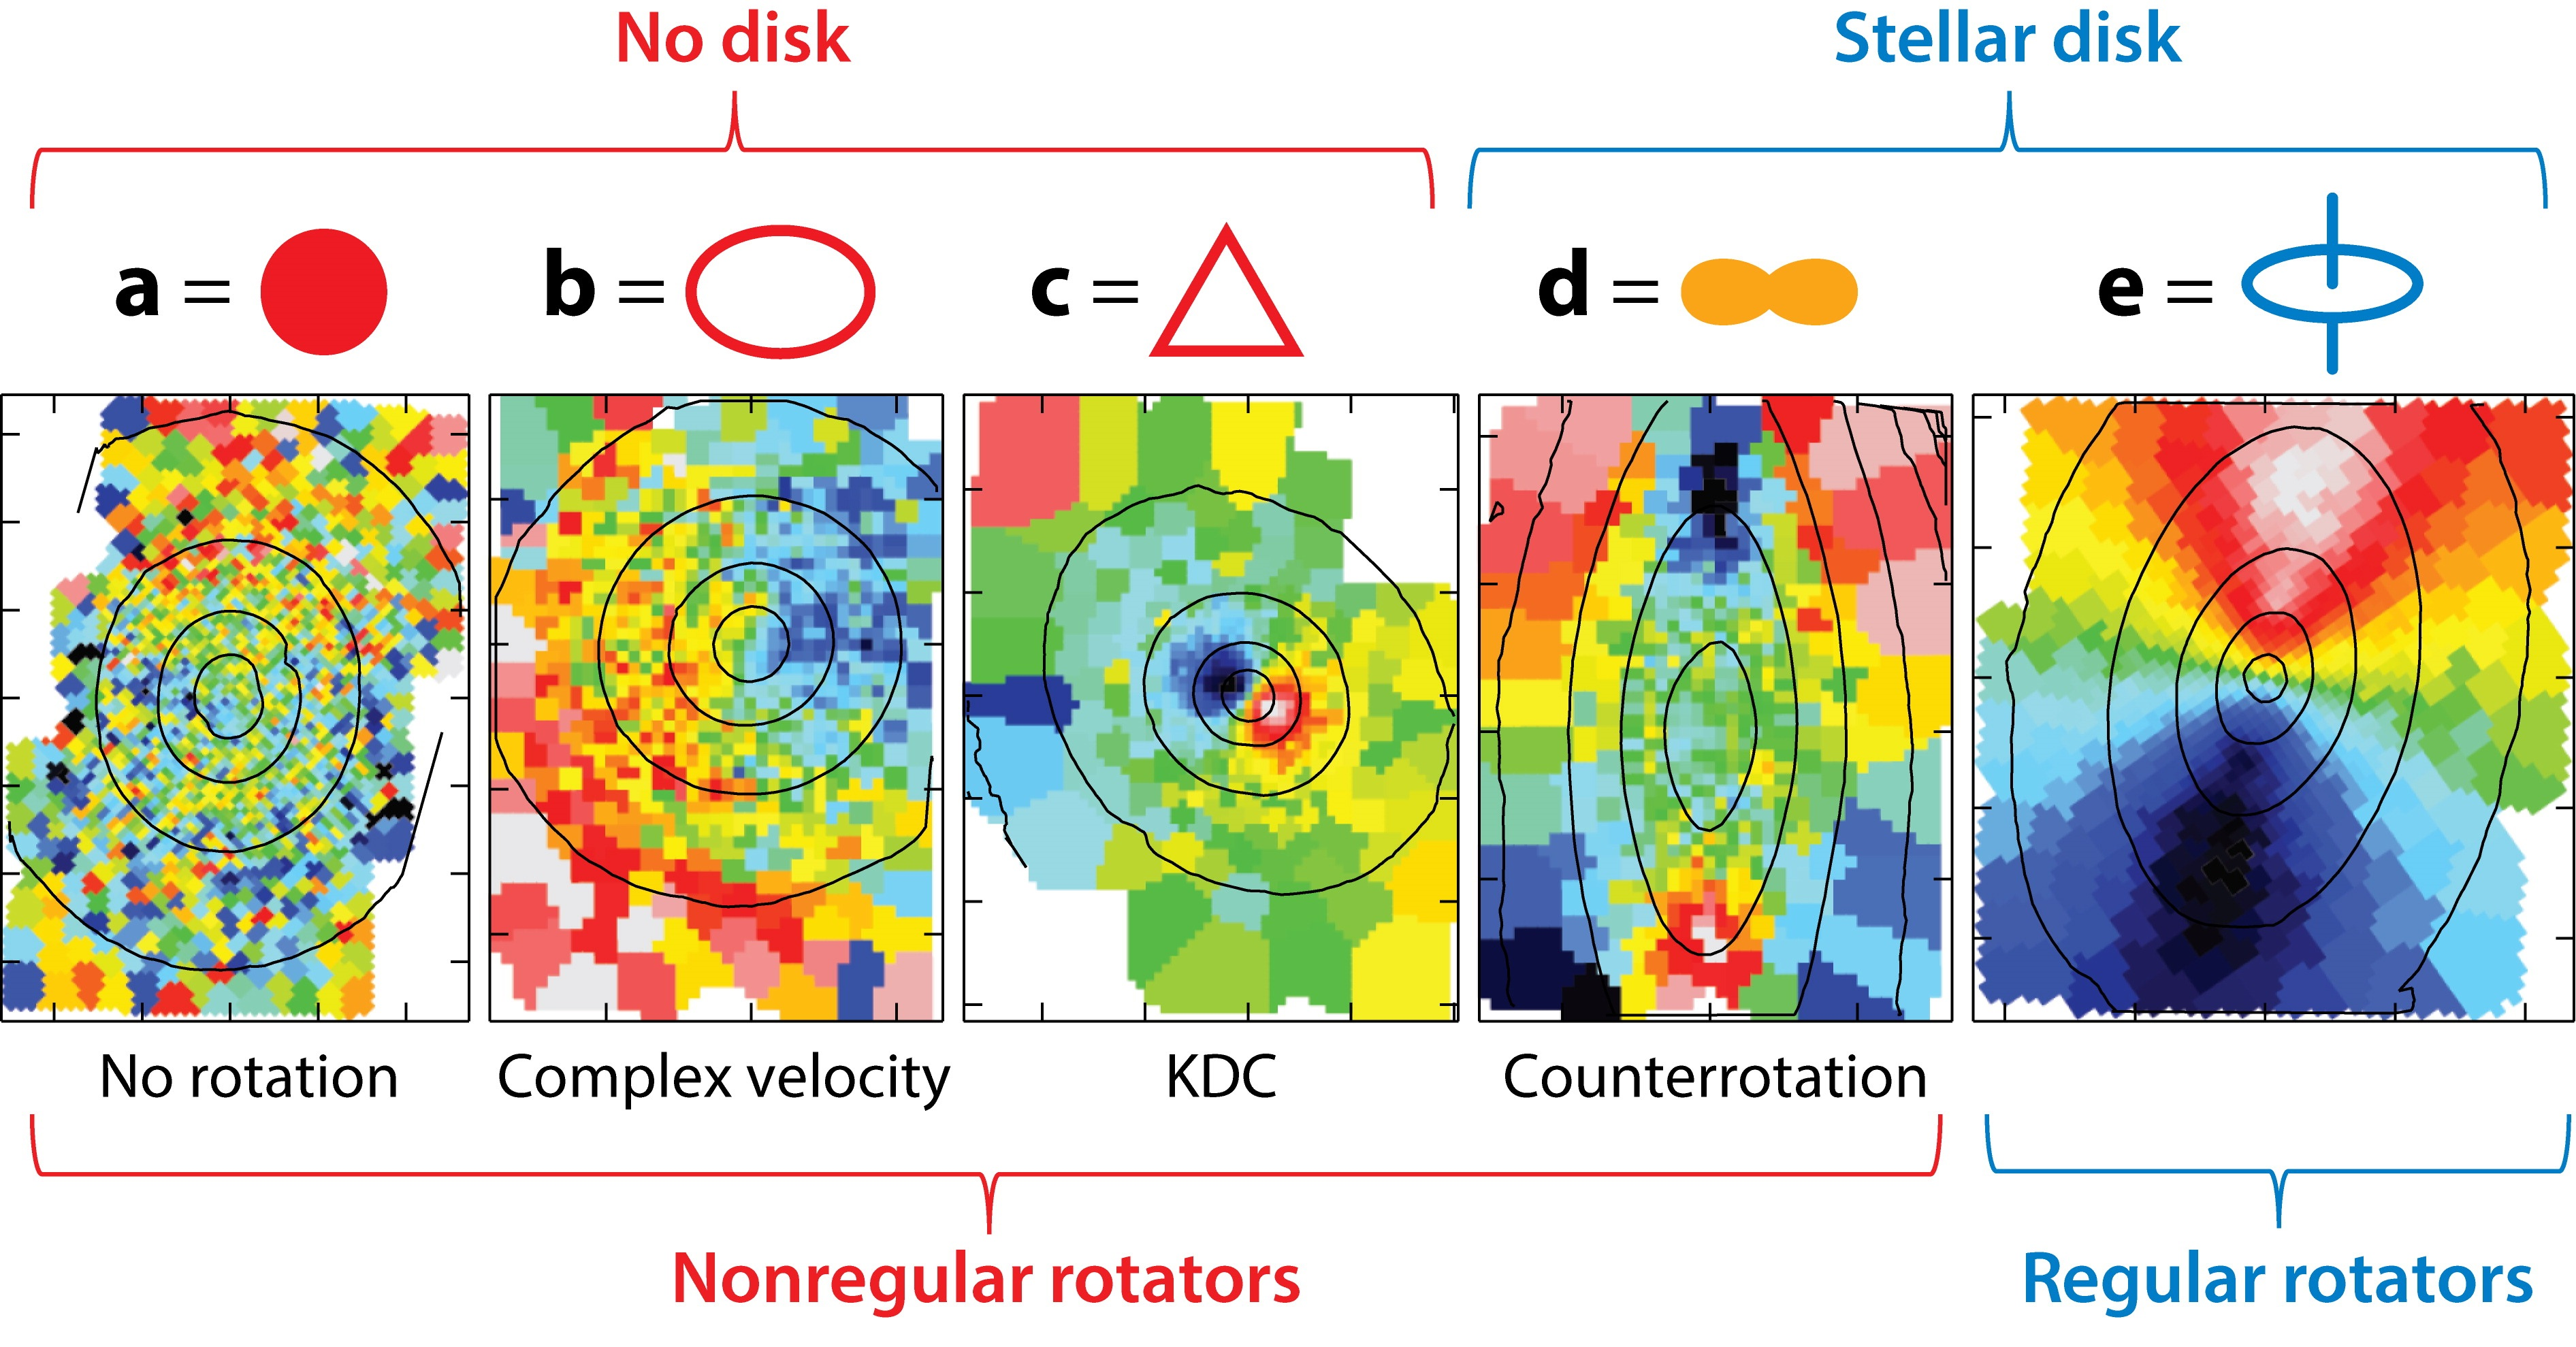
\includegraphics[width=\textwidth]{introduction/substructure.jpeg}
		\caption[Examples of the kinematic substructure classifications]{Figure courtesy of \citet{Cappellari2016}}
		\label{fig:EgSubstructure}
	\end{figure}



\section{Active Galactic Nuclei}
	\label{sec:AGN}
	Much of this section, makes use of the review by \citet{Heckman2014} and the references therein, and we would point readers in the direction of this review if more detail is required. 

	The three main questions that astronomers studying AGN focus on:
	\begin{enumerate}
		\item The origin of the ISM being accreted onto the black hole,
		\item The process by which the ISM is accreted and,
		\item Any processes by which the AGN might effect to the host galaxy (feedback).
	\end{enumerate}
	The final point has been invoked (and indeed seems to be required) in numerous semi-analytic models and numerical simulations to successfully reproduce observations of massive galaxies (\citet{DiMatteo2005, Bower2006, Springel2005} etc.). 

	This section will first look at the different global parameters that can be measured for AGN. After this the two different modes (radiative and jet modes) will be explored.

	\subsection{AGN parameters}
		\label{subsec:AGNparams}

		\subsubsection{Bolometric Luminosity}
			Perhaps the most basic property of any AGN is it's total (bolometric) luminosity. Given the non-spherically symmetric nature of the unified model of AGN, estimating the bolometric luminosity can be a non-trivial task, particularly for obscured (Type 2) AGN. 

		\subsubsection{Black Hole Mass}
			While the black holes are not exclusive to AGN, it is a useful parameter for understanding them and is need for the Eddington limit (see section \ref{subsubsec:Eddington}). Thanks to scale relations, measuring the black hole mass, $M_\text{BH}$ is relatively simple. In this work we use the mass -- stellar velocity dispersion, $\sigma_\ast$ relation (M-\textsigma) from \citet{McConnell2013}:
			\begin{align}
				\log\left(\frac{M_{BH}}{M_\odot}\right) = & \, (8.32 \pm 0.05) + (5.64 \pm 0.32) \log\left(\frac{\sigma_\ast}{200 \mathrm{km \, s^{-1}}}\right) \\
				\intertext{where $\sigma_\ast$ is the luminosity weighted stellar velocity dispersion defined as:} 
				\sigma_\ast^2 \equiv & \, \frac{\int_{R_\text{inf}}^{R_e} \left[\sigma^2(r) + v^2(r)\right] I(r) \mathrm{d}r}{\int_{R_\text{inf}}^{R_e} I(r) \mathrm{d}r}
			\end{align}
			where $I(r)$, $v(r)$ and $\sigma(r)$ are the surface brightness profile, the stellar velocity and stellar velocity dispersion at a radius $r$. $R_e$ is the effective radius: the radius which contains half of the total stellar light, while $R_\text{inf}$ is the radius defining the sphere of influence of the black hole ($R_\text{inf} \equiv \frac{GM_\text{BH}}{\sigma^2}$). In other words, the direct gravitational effect of the black hole is removed from this measure of $\sigma_\ast$. % Does this not mean both M_BH and sigma_* are in the equation defining M_BH and sigma_*? 


		\subsubsection{Eddington Ratio}
			\label{subsubsec:Eddington}
			The Eddington ratio, $L/L_\text{Edd}$, is the ratio of the Bolometric Luminosity to the maximum luminosity the AGN could possibly achieve while still in hydrostatic equilibrium (the Eddington limit), $L_\text{Edd}$. The Eddington limit for pure ionized hydrogen is:
			\begin{equation}
				\frac{L_\text{Edd}}{L_\odot} = \frac{4 \pi G m_p c}{\sigma_T}	\frac{M_\text{BH}}{M_\odot} = 3.3 \times 10^4 \frac{M_\text{BH}}{M_\odot}
			\end{equation}
			where $m_p$ is is the mass of proton and $\sigma_T$ is the Thomson scattering cross-section for an electron on a proton (the ratio $\sigma_T/m_p$ is the opacity of a plasma). 

	\subsection{Radiative Mode}
		\label{subsec:Radiative}
		Radiative mode AGN are thought to show actively growing black holes as accreted matter falls directly into the event horizon. In this case the energy expelled as radiation exceeds that expelled by any jet that may be present (most of the energy of a jet is kinetic): they are typically radiatively efficient with Eddington ratios of 1-100\%. This means that the accretion disk must be geometrically thin. It is thought radiative mode AGN can also drive powerful interstellar winds, capable of terminating star formation and thus moving a galaxy from the blue cloud to the red sequence. 

	\subsection{Jet Mode}
		\label{subsec:Jet}
		In jet mode, the dominant form of emitted energy away from the black hole is the kinetic energy of the material that makes up the jet. Jet-mode AGN can be directly observed feeding-back to their host galaxies: they often terminate at shocks (hot spots), which make up the walls to cavities in the hot (X-ray) component of the host galaxy.

		Jet mode AGN tend to be radiatively inefficient with Eddington ratios of $<$1\%. This implies that the inner most accretion disk must be geometrically thick, with an inflow time that is much less that the radiative cooling time scale. These are known as a advection-dominated accretion flow (ADAF). It is possible that there is a thin disk beyond this (further from the black hole) but it must be truncated by the thick disk. Such a system is capable of launching a jet. 

		It is thought that the duty cycle of a jet is very short: it is turned on for very short periods of time, before turning off for an extended period. When the jet is turned off or only very weakly present, the galaxy may present as containing a low ionization nuclear emission-line region (LINER). It is worth noting that while the most powerful LINERs are likely to be low-luminosity AGN, many are not: they belong to a new category known as LIERs (the emission-line region is not nuclear - i.e. LINER but without the 'N') \citep{Sarzi2005, Sarzi2010, Singh2013, Belfiore2016a}. Such emission is mostly attributed to ionization from radiation from post-asymptotic giant branch (AGB) stars. 

		As stated above, most RGs result from synchrotron emission from the relativistic plasma within the jet, moving in the magnetic field of the galaxy. This means that all such RGs can be considered a detection of a jet (we ignore the very low radio luminosity galaxies that result from high levels of circumnuclear star-formation). RGs are always jet mode AGN, except at the highest radio luminosities where the bright radio jet is dominated (in terms of energy output) by the brighter still accretion disk. These are radiative mode AGN.

		There is still much speculation on the fuel (and origin) for jet mode AGN, though the consensus is swinging back in favor of an internal origin. Many people advocate hot gas as being the ultimate original fuel: some suggest that this could be directly accreted through Bondi accretion, a simple model where gas in accreted in a spherically symmetric manner directly from the hot phase onto the black hole; while some invoke a cooling mechanism to allow the x-ray gas to cool such that it condenses into molecular (cold) gas before accretion. Others point to a higher higher detection rate of dust and molecular (cold) gas in RGs compared to the general population suggesting that cold gas from either internal reservoirs or accreted from outside that gas may be the fuel.



\section{The Southern Sample}
	\label{sec:Sample}
	In order to study RGs in better detail we here set out a sample of 11 galaxies in the Southern Hemisphere. This sample is similar to the B2 sample of Northern Hemisphere galaxies. 

	We use the Parkes 2.7GHz survey as a parent sample. This survey found radio sources with an optical counterpart. We discard any galaxy where the host has a redshift less than 0.03. The key selection criteria are shown in table \ref{tab:selection}. It is worth noting that both the radio and optical limits are apparent measurements and as such this is not a volume limited sample.

	\begin{table}
		\centering
		\caption{Key selection criteria.}
		\label{tab:selection}
		\begin{tabular}{l l}
			\hline
			\hline
			Observability:				& $-17\degree < \delta < -40\degree$ \\
			2.7GHz flux density: 		& $S_\text{2.7GHz} \ge 0.25 \text{Jy} $ \\
			V-band apparent magnitude: 	& $m_V \le 17.0 $ \\
			Redshift: 					& $z < 0.03$ \\			
			\hline
			\hline
		\end{tabular}
	\end{table}

	These criteria selects 11 galaxies (hereafter refered to as the Southern Sample). The key observed characteristics are sumerised in table \ref{tab:sample}, while the derrived characteristics are given in table \ref{tab:sampleDerrived}.

	\begin{table}
		\centering
		\caption{Key sample characteristics: Col.1: host galaxy name, Col.2: radio source name (from PKS catalogue), Col.3: Redshift, Col.4: 1.4GHz flux density, Col.5: K-band absolute magnitude.}
		\label{tab:sample}
		\begin{tabular}{l l l l l}
			\hline
			\hline
			Host galaxy	& Radio source 	& z 		& $S_\text{1.4GHz}$	& $M_k$ \\
						& PKS ID 		& 			& mJy 				& mag \\
			\hline 
			ESO 443-G024 & 1258-321 	& 0.01703	& 1465 				& -25.87 \\ 
			IC 1459 	& 2254-367 		& 0.00565 	& 1274 				& -25.27 \\
			IC 1531 	& 0007-325 		& 0.02553 	& 582 				& -25.70 \\
			IC 4296		& 1333-33 		& 0.01248 	& 64282 			& -26.18 \\
			NGC 612 	& 0131-36 		& 0.02954 	& 4980 				& -26.01 \\ % Check pks number
			NGC 1316 (Fornax A) & 0320-37 & 0.00591 & 314 				& -26.44 \\
			NGC 1399 	& 0336-35 		& 0.00472 	& 632 				& -25.25 \\
			NGC 3100 	& 0958-314 		& 0.00879 	& 541 				& -24.85 \\
			NGC 3557 	& 1107-372 		& 0.01016 	& 777 				& -26.08 \\
			NGC 7075 	& 2128-388 		& 0.01819 	& 963 				& -24.98 \\
			--			& 0718-34 		& 0.02897 	& 2050 				& -25.59 \\
			\hline
			\hline
		\end{tabular}
	\end{table}



	\begin{table}
		\centering
		\caption{Derrived characteristics of the Southern sample: Col.1: galaxy name, Col.2: Radio spectral index. The data spectral index is found from a straight line fitted to }
		\label{tab:sampleDerived}
		\begin{tabular}{l l l l l}
			\hline
			\hline
			Host galaxy	& \nu $ 			\\
						& 					\\
			\hline 
			ESO 443-G024 & $-0.56 \pm 0.08$	\\
			IC 1459 	& $0.25 \pm 0.06$ 	\\
			IC 1531 	& $-0.33 \pm 0.03$ 	\\
			IC 4296		& $-1.52 \pm 0.27$ 	\\
			NGC 612 	& $-1.05 \pm 0.24$ 	\\
			NGC 1316 	& $-4.7 \pm 2.1$ 	\\
			NGC 1399 	& $-0.65 \pm 0.66$ 	\\
			NGC 3100 	& $-0.40 \pm 0.03$ 	\\
			NGC 3557 	& $-0.72 \pm 0.13$ 	\\
			NGC 7075 	& $-0.90 \pm 0.06$ 	\\
			PKS 0718-34 & $-0.63 \pm 0.06$ 	\\
			\hline
			\hline
		\end{tabular}
	\end{table}
